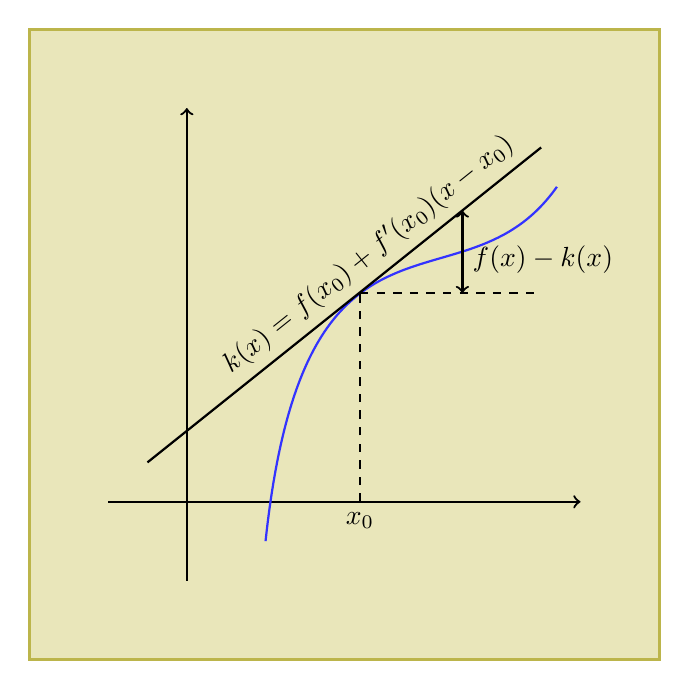
\begin{tikzpicture}
  \draw[draw = olive!60, fill = olive!20, very thick]
    (-2, -2) rectangle (6, 6);

  \draw[->, thick] (0, -1) -- (0, 5);
  \draw[->, thick] (-1, 0) -- (5, 0);

  \draw[thick, color = blue!80]
    (1, -0.5) .. controls (1.5, 4.2) and (3.5, 2.3) .. (4.7, 4);

  \draw[thick] (-0.5, 0.5) -- (4.5, 4.5)
    node[pos = 0.6, above, sloped] {\(k(x) = f(x_0) + f'(x_0) (x - x_0)\)};
  \draw[dashed, thick] (2.2, 0) -- (2.2, 2.65)
    node[pos = 0, below] {\(x_0\)};
  \draw[dashed, thick] (2.2, 2.65) -- (4.5, 2.65);

  \point{2.2, 2.65};
  \draw[<->, thick] (3.5, 2.65) -- (3.5, 3.7)
    node[pos = 0.4, right] {\(f(x) - k(x)\)};

\end{tikzpicture}